\documentclass[14pt]{book}
\usepackage{pythontex}
\usepackage{polyglossia}
\usepackage{hyperref}
\usepackage[listings,skins,xparse]{tcolorbox}
\usepackage{float}
\usepackage{graphicx}

\setdefaultlanguage[calendar=islamic,numerals=maghrib]{arabic}
\setotherlanguage{english}
\newfontfamily\arabicfont[Script=Arabic,Scale=1.3]{Amiri}
\newfontfamily\arabicfonttt{Tahoma}


% creating new input file for customized colored box
\newtcbinputlisting[auto counter,number within=section]{pythoncode}[1]{enhanced,title=\flushright{\thetcbcounter \textarabic{مثال رقم }} ,fonttitle={\bfseries\large},listing file={#1},listing options={language=python,numbers=left,numbersep=2.5mm,keywordstyle=\color{blue!90!black}\bfseries,commentstyle={\color{green!45!black}\itshape},stringstyle=\color{red!75!black},
showstringspaces=false,basicstyle=\normalsize},listing only,colframe=green!30!blue!60!black,colback=white,before skip=20pt,after skip=20pt,
overlay={\begin{tcbclipinterior}\fill[green!30!blue!15!white] (frame.south west) rectangle ([xshift=4mm]frame.north west);\end{tcbclipinterior}}}

\newtcolorbox{mybox}{after skip=20pt,  before skip=20pt}


\title{\Huge\textsc{مبادئ البرمجة بلغة بايثون}}
\author{احمد سالم الصاعدي} 
%\includeonly{introduction}
%\includeonly{aboutpython}
\includeonly{python_basics}
%\includeonly{pythonlists}
%\includeonly{pythonloops}
%\includeonly{pythondecisions}
%\includeonly{pythonmodules}
%\includeonly{pythonoop}
%\includeonly{pythongui}

\begin{document}
\maketitle
\tableofcontents
\chapter*{مقدمة}
الحمد لله الذي تتم بفضله الصالحات واصلي وأسلم على خير البشر نبينا محمد صلى الله عليه وسلم وعلى آله وصحبه الطيبين الطاهرين. اما بعد:
فلقد لاحظت خلال فترة تعلمي للغة بايثون افتقار المكتبة العربية الى كتاب مكتمل يشرح مبادي هذه اللغة بشكل منظم وبسيط. فعقدت العزم على تأليف هذه الكتاب وذلك لما رايته من الأهمية بمكان ان يتعلم القارئ العربي هذه اللغة والتي أصبحت اللغة البرمجية المحبوبة لدي الكثير من العلماء والباحثين والمهندسين. فمعظم جامعات العالم اليوم أصبحت تدرسها لطلابها فهي لغة برمجة مشهورة , قوية ويمكن استخدامها في مجالات عدة. لذلك اردت ان يكون هذا الكتاب لبنة أولى للمساهمة في تعليم هذه اللغة. الذي امل ان يتم تدريسها في مدارسنا الحكومية في مراحل مبكرة كالمتوسطة والثانوية وذلك لان الأجيال الحالية على اطلاع واسع بالتقنية وخصوصا الكمبيوترية منها. فهي اصحبت قدرة على تعلمها والاستفادة منها دون مشقة. وبما ان هذا العمل بشري المصدر فانه لا يصل الى درجة الكمال لذلك ارجو ممن سنحت له الفرصة لقراءة هذا الكتاب ان يساهم في تحسين هذا الكتاب بارسال ملاحظاته الى ايميل المؤلف 
ahmad.alsaadi@kaust.edu.sa
 الذي يعدكم على انه سوف يعمل على اخذها في الاعتبار متى ما سنحت الفرصة لاصدار طبعة جديدة لهذا الكتاب.
\chapter{نبذه عن لغة بايثون}
\noindent
أعتقد انه من الاهمية بمكان ان يتعلم كل واحد منا لغة البرمجة وذلك لانها  تساعدنا على تعلم طريقة التفكير الصحيحة
\begin{flushright} 
ستيفن جوبز
\end{flushright}
\rule{\textwidth}{1pt}
\section{تعريف لغة بايثون }
بايثون لغة برمجية مفتوحة المصدرسهلة التعلم يمكن الاعتماد عليها في كتابة الكثير من التطبيقات البرمجية القوية. واكبر دليل على ذلك هو استخدام وكالة الارصاد الامريكية ناسا وشركة قوقل وياهو وغيرها من الشركات الكبرى لهذه اللغة في بناء برامجهم المختلفة. 
\section{نشئة لغة بايثون}

كانت بدايات نشئة هذه اللغة في هولندا على يد شخص يدعي جويدو فان روزم
\textenglish{(Guido van Rossum)}
 في نهاية الثمانيات الميلادية من القرن العشرين. لكن لم يتم الاعلان عنها الا في عام ١٩٩١م.   ويعتبر فتح مصدر هذه اللغة من اهم الاسباب التي ادت الى زيادة شهرتها وذلك من خلال تكوين مجتمع برمجي نشط حولها اسهم في  انشاء مكتبات كثيرة سهلت على المطورين الاخرين بناء تطبيقاتهم بسرعة و سهوله فائقة مقارنة باللغات البرمجية الاخري.

\section{ مزايا لغة بايثون}
للغة بايثون مزايا عدة جعلت منها اللغة المفضلة الاولى لدى كثير من المبرمجين ومن بين اهم هذه المزايا نذكر:
\begin{enumerate}
\item
سهولة تراكيبها اللغوية: فاكوادها البرمجية تكتب بطريقة قريبة جدا من اللغة الانجليزية. لذلك نجدها لاتشكل اي عائق امام أي مبرمج ان يفهم الأكواد المكتبوبة من قبل مبرمجين اخرين عندما يستدعي الامر صيانة تلك الاكواد اوتحديثها.
\item
المرونة: يمكن تشغيل وتطوير البرامج المكتوبة بلغة بايثون على معظم انظمة التشغيل المعروفة. فالأكواد التي تم تطويرها على نظام ويندوز يمكن تشغيلها على نظام ماك ولينكس والعكس صحيح دون الحاجة الى اعادة بناء الأكواد
 .(compiling)
\item
كثرة المكتبات: يعتبر توفر المكتبات من اهم المزايا التي تقدمها اللغة للمبرمجين لتزيد من فعاليتهم في بناء التطبيقات. لذلك عند تنصيب اصدارة بايثون نجد انها تحتوي على مكتبات قياسية كثيرة بعضها يعتبر جزء لا يتجزء من تراكيب اللغة كمكتبة الارقام والقوائم وبعضها الاخر يعمل على تسهيل التعامل مع انظمة التشغيل اما الجزء الاكبر من هذه المكتبات فهو اختياري يتم استيراده متى ما دعت الحاجة لذلك. كما ان هناك مكتبات اخري تحتاج الى تنصيب قبل ان يتمكن المبرمج من استيرادها واستخدامها في برنامجه. وهذه المكتبات مجانية ويمكن تحميلها وتنصيبها اما من الموقع الخاص بالمطورين لهذه المكتبة او من موقع
 \href{http://pypi.python.org}{http://pypi.python.org}
  والذي يحتوي حتى وقت كتابة هذه السطور على 69478 مكتبة مجانية جاهزة يمكن استخدامها في بناء التطبيقات المختلقة.
\item
التكامل مع لغات برمجية اخرى: يمكن استخدام بايثون كلغة مساندة تمكن المستخدم لبرنامج مكتوب بلغة سي (C) او سي بلس بلس (C++) مثلا من زيادة او تعديل خصائص ذلك البرنامج ليتناسب مع احتياج المستخدم. ومن أقرب الامثلة على ذلك هو استخدام لغة بايثون في برنامج فري كاد (FreeCAD) كلغة برمجة نصية لتحكم بكافة خصائص البرنامج ووظائفه.
\end{enumerate}

\section{اصدارت بايثون}
هناك اصدارتان لبايثون. الإصدارة الأولى تعرف ببايثون 2 وهي الاقدم والاصدارة الاخرى تدعى بايثون 3 وهي الاحدث.
\section{تنصيب مفسر لغة بايثون}
\subsection{تنصيب بايثون على نظام ويندوز}

اذا كنت تستخدم اي من انظمة ميكروسوف ويندوز سوا القديم منها او الحديث فانك تحتاج الى تنصيب مفسر لغة بايثون على هذا النظام. واليك الخطوات التالية التي 
تساعدك على عمل ذلك:
\begin{enumerate}
\item
حمل مفسر بايثون من الموقع التالي:
\href{https://www.python.org/downloads/}{http://python.org/downloads/}
يمكنك الاختيار بين احدى الاصدارتين ٢ او ٣. في هذا الكتاب سوف نستخدم الاصدارة ٢. ليس هناك اختلاف جذري بين الاصدارتين في كتابة اكواد اللغة وسوف نشير الى مواضع الاختلاف متى ما تطرقنا الي ذلك عند شرحنا لتراكيب لغة بايثون.
\item
نصب مفسر بايثون باتباع التعليمات الموجودة في برنامج التنصيب
\item
جهز بيئة ويندوز للتعرف على مفسر بايثون باتباع الخطوات التالية:
\end{enumerate}
\subsection{تنصيب بايثون على ابل ماك}
يأتي نظام تشغيل ماك وقد نصب عليه مفسر بايثون ذو الاصادرة رقم ٢. ويمكن التأكد من ذلك باتباع الخطوات التالية:
\begin{enumerate}
\item
قم بتشغيل محرر الاوامر في الماك "terminal" باجدى الطريقتين التاليتين:
\begin{enumerate}
\item
الذهاب الى ملف التطبيقات "Application" من ادارة الملفات "Finder" واختيار محرر الاوامر "terminal" من هناك
\item
الضغط على زر المسافة و زر الاوامر "cmd" في آن واحد تم البحث عن برنامج "terminal"
\end{enumerate}
\item
اكتب في محرر الاوامر الامر التالي بعد علامة الدولار \$ :
 
\begin{figure}[H]
  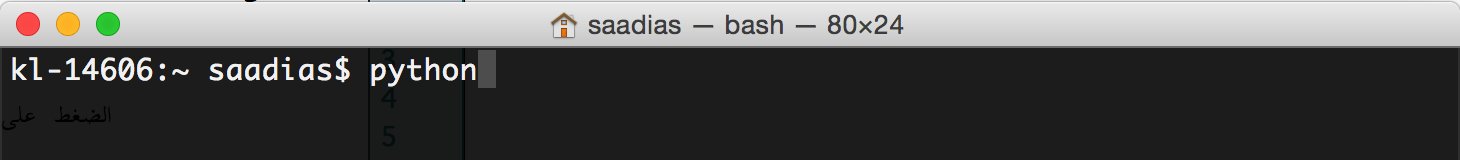
\includegraphics[width=\linewidth]{figures/startpython.png}
  \caption{طريقة بدء مفسر بايثون من محرر الاوامر في الماك}
  \label{fig:startpython}
\end{figure}
بعد الضغط على زر الادخال سوف تحصل على الاتي:

\begin{figure}[H]
  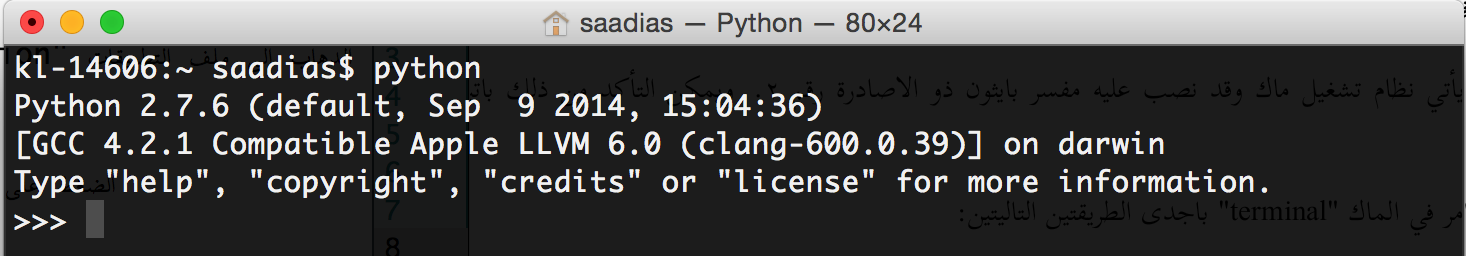
\includegraphics[width=\linewidth]{figures/startpython2.png}
  \caption{بداية تشغيل مفسر اوامر بايثون}
  \label{fig:startpython2}
\end{figure}

وهو يدل على ان بايثون منصب على هذا الجهاز وهو من الاصدارة رقم ٢.٧.٩  كما ان المفسر يبدا مباشرة بالوضع التفاعلي والذي يبدأ بمؤشر خاص 

\end{enumerate}
\subsection{تنصيب بايثون على نظام لينكس (اوبينتو)}
:

كما هو الحال مع نظام ماك فان نظام اوبينتو لينكس يحتوي على مفسر بايثون وهو كذلك من الاصدارة رقم ٢. لتأكد من وجود بايثون على ابيونتو يمكن اتباع نفس الخطوات التي عملنها مع نظام الماك.

\begin{figure}[H]
  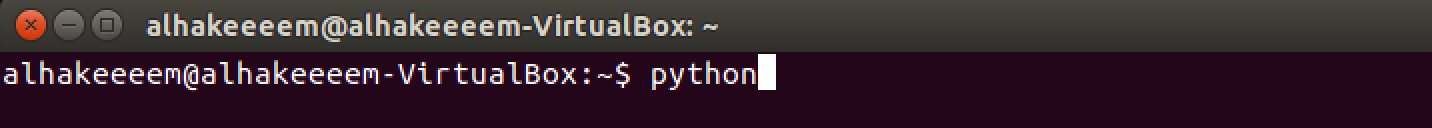
\includegraphics[width=\linewidth]{figures/ubintupython.png}
  \caption{طريقة تشغيل مفسر بايثون في نظام لينكس اوبينتو}
  \label{fig:startpython2}
\end{figure}

\begin{figure}[H]
  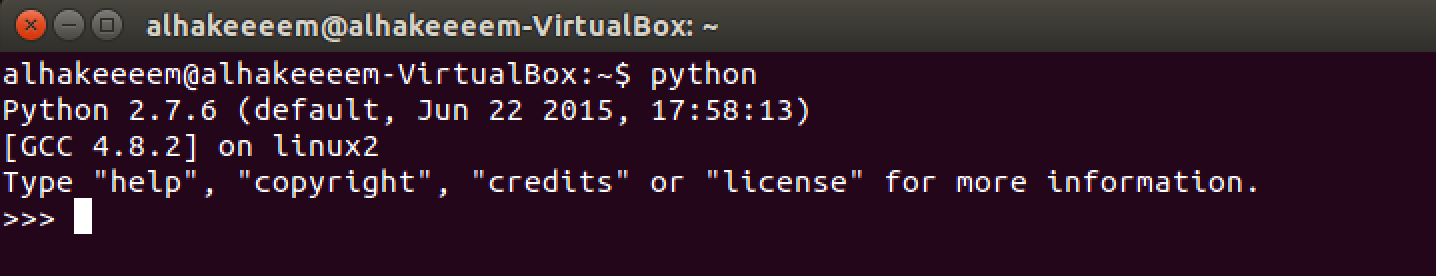
\includegraphics[width=\linewidth]{figures/ubintupython2.png}
  \caption{بدء تشغيل مفسر بايثون في نظام لينكس اوبينتو}
  \label{fig:startpython2}
\end{figure}
هنا ياتي بايثون باصدارة رقم ٢.٧.٦ وكذلك يبدأ بالوضع التفاعلي.		

\section{طريقة كتابة الكود البرمجي في بايثون}
هناك طريقتان يمكن بهما كتابة الاكواد البرمجية لبايثون:
\begin{enumerate}
\item
الطريقة التفاعلية:
وهي الطريقة التي تمكن المستخدم من رؤية نتاتج الامر البرمجي مباشرة بعد الضغط على زر الادخال. وهذه الطريقة تجعل من بايثون اشبه بالالة الحاسبة حيث يتم الحصول على النتائج مباشرة بعد معالجتها من قبل المفسر.لتاكد من ادراكك لهذه الطريقة يمكنك تجربة كتابة الاكود الاتية بعد مؤشر بايثون الخاص وضغظ زر الادخال بعد كل سطر.
\begin{enumerate}
\item

print "welcome to python world"
\item
2+2
\item
x=7
\item
print x
\end{enumerate}
اذا قمت بادخال الاوامر السابقة بشكل صحيح فانك سوف تحصل على النتائج الموضحة في الشكل ادناه:
\begin{figure}[H]
  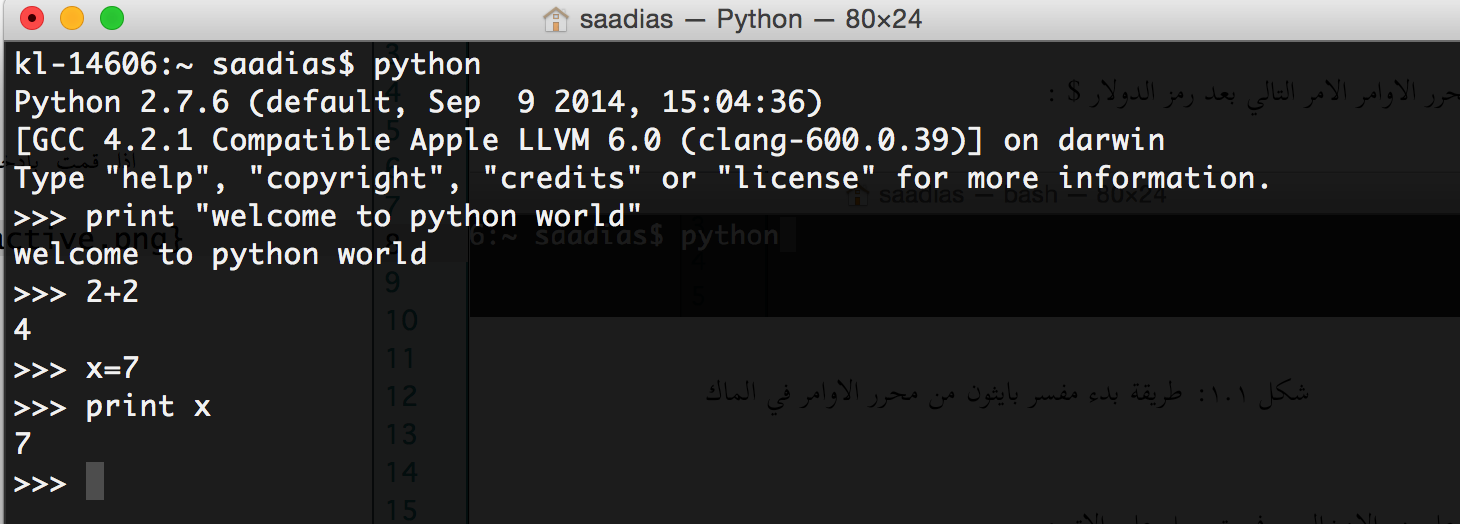
\includegraphics[width=\linewidth]{figures/interactive.png}
  \caption{الوضع التفاعلي لمفسر بايثون}
  \label{fig:startpython2}
\end{figure}
اذا لم تزل غير متاكد من استيعابك لهذه الطريقة يمكنك زيارة موقع الكتاب ومشاهدة الفديو التوضيحي لهذه الطريقة.
\item
استخدام محرر النصوص:
يأتي مع مفسر بايثون محرر نصوص يدعى "ايدل" ويمكن تشغيلة بكاتبة الامر idle من خلال محرر الاوامر في ماك ولينكس. قد يكون idle غير منصب على نظام لينكس اوبينتو لذلك سوف تظهر له تعليمات تبين لك طريقة تنصيبه كما في الشكل التالي:
\begin{figure}[H]
  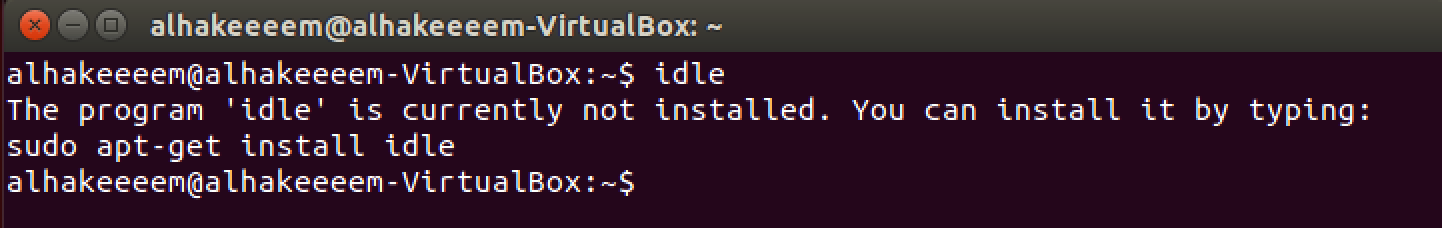
\includegraphics[width=\linewidth]{figures/installidle.png}
  \caption{idle غير منصب على نظام لينكس اوبينتو}
  \label{fig:startpython2}
\end{figure}
ويكمن القيام بعملية التنصيب بادخال الامر التالي في محرر الاوامر:
\begin{flushleft}
sudo apt-get install idle
\end{flushleft}
سوف يطلب منك نظام ادخال كلمة المرور قبل تنفيذ امر التنصيب قم بادخال كلمة المرور الخاصة بك ثم اضغط على زر الادخال. عند اتمام علمية التنصيب ادخل الامر idle لتشغيل محرر النصوص الخاص ببايثون. سوف تظهر له نافذة مستقلة مشابهه لمحرر بايثون التفاعلى السابق انظر الشكل س. حيث يكمنك ان تحصل على نفس النتائج اذا قمت بادخال اومر بايثون انفة الذكر.
\begin{figure}[H]
  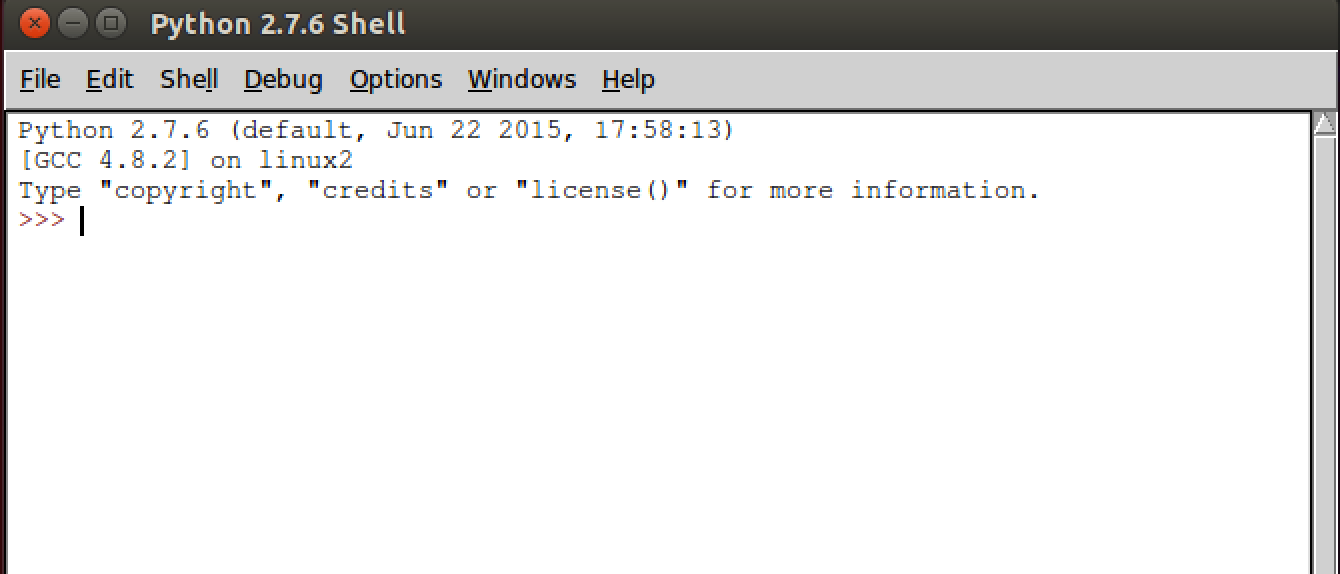
\includegraphics[width=\linewidth]{figures/idle.png}
  \caption{محرر نصوص بايثون}
  \label{fig:startpython2}
\end{figure}
\end{enumerate}
\chapter{اساسيات لغة بايثون}
بعد ان تأكدنا من ان نظام التشغيل الذي نعمل عليه يحتوي على احدى اصدارات لغة بايثون يمكننا الان ان نبدأ رحلة التعلم والتى اتمنى ان تكون حافلة بالمتعة والفائدة.\\
\section{أهداف الباب}
عند اتمام هذا الباب يجب ان يكون لديك المام بعدة مبادئ اساسية عن لغة بايثون والتي من اهمها:
\begin{enumerate}
\item
بايثون لغة تفرق بين كون احرف التركيب اللغوي مكتوبة باحرف صغيرة ام كبيرة وتتعامل معها بشكل مختلف
\item
بايثون تهتم بعدد المسافات المتروكة قبل بداية كل سطر برمجي
\textenglish{(indentation)}
\item
كيفية طباعة نص على شاشة الكمبيوتر
\item
طريقة تدوين الملاحظات على الكود البرمجي
\textenglish{(comments)}
\item
اجراء العمليات الحسابية الاساسية 
\item
طريقة كتابة المتغيرات
\textenglish{(variables)}
 لتخزين البيانات من اجل تحليلها ومعالجتها
\item
أنواع البيانات في بايثون
\textenglish{(data types)}
\item

\end{enumerate}

\section{ الاحرف الصغيرة $\neq$ الاحرف الكبيرة:}
لغتنا العربية الجميلة لاتحوي على مفهوم الحروف الصغيرة والكبيرة بعكس ما هو موجود في اللغة لانجليزية. وبما ان لغة بايثون مكتوبة باللغة الانجليزية فان هذه اللغة تهتم بما اذا كان الكود البرمجي او جزء منه مكتوب بالاحرف الصغيرة او الكبيرة. فالامر print مثلا يكتب بالاحرف الصغيرة كما في المثال التالي:\\
\begin{english}
\begin{tcolorbox}
\begin{pyconsole}
print "welcome to python"
\end{pyconsole}
\end{tcolorbox}
%\pythoncode{code/small_letters.py}
\end{english}

ولكن عندما نحاول كتابته احد حروف هذا الامر بحرف كبير فان مفسر لغة بايثون يعطينا خطأ مخبرا ان التركيب اللغوي غير صحيح كما في المثال التالي:
\begin{english}
\begin{tcolorbox}
\begin{pyconsole}
prinT "welcome to python"
\end{pyconsole}
\end{tcolorbox}
%\pythoncode{code/capital_letters.py}
\end{english}
ربما قد تبادر الى اذهان البعض الان ان تذكر وضع حالة الاحرف ما اذا كانت صغيرة ام كبيرة  يعد امرا شاقا. لكن علينا ان نتادرك الموقف بسرعة ونبين لهم ان هناك ضوابط وضعت من قبل مطويرين لغة بايثون تجعل من تذكر وضع حالة الاحرف غاية في السهولة.
\\
\\
\textbf{الضابط الاول:}
 ان جميع اوامر لغة بايثون دائما تكون مكتوبة بالاحرف الصغيرة. 
\textbf{الضابط الثاني:}
 ان الاحرف الكبيرة  تستخدم فقط عند كتابة الثوابت. 
 \\
 \\
 قد لا يكون هذا الامرواضحا بما فية الكفاية الان ولكن أعدك ان أوضح هذه المسألة بعد ان أتطرق الى المفاهيم  الاساسية في لغة بايثون. فكل ما عليك فهمه الآن هو ان لغة بايثون تفرق بين حالة الاحرف الصغيرة والكبيرة في تراكيبها اللغوية.
\\
\section{ترك مسافات في تركيب بايثون اللغوي}
في حين ان لغات البرمجة الاخرى تستخدم مصطلحات واقواس لتحديد بداية ونهاية الاجزاء  الداخلية للكود البرمجي فان لغة بايثون تتبع نظام ترك المسافات عند بداية كتابة السطر البرمجي لاداء نفس المهمة. فلغة جافا تستخدم الاقواس لتحديد جزئية الكود الداخلي و علاقته ببقية الاجزاء كما في المثال التالي:
بينما لغة بايثون تعمد الى ترك مسافة عند بداية كتابة الجزء الداخلى للكود لتجديد مداه وعلاقتة بالاجزاء الاخرى كما في المثال التالي:
ليس من المهم ان تفهم وظيفة الكود البرمجي السابق الان لاننا سوف نتطرق اليه في وقت لاحق ولكن المهم ان تعرف ان لغة بايثون تهتم بترك مسافات عند بداية كتابة الاسطر البرمجية لتحديد الاجزاء الداخلية من الكود.فعند كتابة برنامج من سطر واحد مثلا فان ترك اي مسافة قبل بداية السطر البرمجي يجعل مفسر بايثون يرفض التركيب اللغوي و يظهر رسالة تبين سبب المشكلة هو ترك مسافة عند بداية كتابة السطر البرمجي في موضع لايستدعي ترك اي مسافة. يمكنك التأكد من هذا بترك مسافة قبل السطر البرمجي كما في المثال التالي:
\begin{english}
\begin{tcolorbox}
$>>>$     print "hello" \\
    \\
  File "<pyshell\# 2>", line 1 \\
    \quad print "hello"  \\
   $\^$ \\
IndentationError: unexpected indent \\
$>>>$ 
\end{tcolorbox}
\end{english}
لكن ترك مسافة في اي موضع اخى من السطر ليس له اي تأثير على التركيب اللغوي. كما يجب الاشارة الى ان ترك اسطر فارغة بين اسطر الكود البرمجي ليس له اي تأثير يذكر ايضا. سوف نعاود الحديث عن ترك المسافات عندما نبدأ الحديث عن الحلقات التكرارية والدوال في بايثون حيث تستدعى الحاجة للحديث عن ترك مسافات عند كتابة هذه التراكيب اللغوية.
\section{طباعة نص على شاشة الكمبيوتر:}
كما هو المعتاد في تعلم اي لغة برمجة جديدة فان البدء دايما ما يكون بتعلم كيفية طباعة نص على شاشة الكمبيوتر. وسوف نسير على هذا العرف نحن هنا ايضا. فامر الطباعة على الشاشة في بايثون يكون باسيتخدام الامر print متبوعا بما يراد طباعتة. وبما اننا في بداية المشوار ولم نتطرق لمفوهم المتغيرات فسوف نبدأ بطباعة النصوص اولا. فالسطر البرمجي  التالي يقوم بطباعة
welcome to python
 على الشاشة:

print "welcome to python"

لاحظ ان هناك قواعد يجب معرفتها عند طباعة النصوص ومن بين هذه القواعد مايلي:
\begin{enumerate}
\item
يمكن استخدام علامات التنصيص الاحادية (’) او الثنائية (") او الثلاثية (’") لتحيط بالنص المراد طباعته على الشاشة. مع ملاحظة انه يجب ان تسخدم نفس علامة التنصيص في بداية النص واخره وعدم الخلط بينها. كما هو موضح في المثال التالي:

\item
علامة التنصيص الاحادية والثنائية تستخدم لكاتبة نصوص من سطر واحد بينما علامة التنصيص الثلاثية تسمح بطباعة اكثر من سطر. كما في المثال التالي:
\item
يمكن استخدام رمز التجاهل "\" لتمكين علامة التنصيص الاحادية والثنائية من طباعة اكثر من سطر على الشاشة. كما في المثال التالي:

\item
يمكن استخدام علامة تنصيص او اكثر داخل علامتي تنصيص ولكن بعد التأكد من ان علامة التنصيص الداخلية مختلفة عن علامة التنصيص المستخدمة في بداية ونهاية النص. كما يمكن استخدام رمز التجاهل المشار اليه سابقا لاداء نفس الوظيفة.  كما ماهو موضح في الامثلة التالية:

\end{enumerate}

\section{تدوين الملاحظات}
تسمح لغة بايثون كغيرها من لغات البرمجة للمبرمج بان يكتب ملاحظاته داخل الكود البرمجي من اجل ان تساعدة على تذكر وظيفة الكود البرمجي او من اجل اعطاء شروحات وافيه للمبرمجين الاخرين الذين قد يعملون على صيانة وتطوير الكود البرمجي في المستقبل. ويمكن كتابة ملاحظة من سطر واحد في اي مكان من الكود البرمجي ولكن بعد ان يسبق الملاحظة علامات الهاشتاق 
(\#)
كما في المثال التالي:
\begin{english}
\pythoncode{code/basics1.py}
\end{english}
كما يمكن كتابة ملاحظة متعددة السطور باستخادام علامة التنصيص الثلاثية كما في المثال التالي:
\begin{english}
\pythoncode{code/basics2.py}
\end{english}

%**************** Data types********
%**********************************
\section{انواع البيانات في بايثون}
تنقسم انواع البيانات في بايثون لثلاثة اقسام. بيانات رقمية وبيانات منطقية وبيانات نصية. البيانات الرقمية تش
\begin{enumerate}
\item
البيانات المنطقية
\textenglish{Boolean}
: وهي البيانات التي تحتوي على قيمتين فقط صح
\textenglish{True} 
و خطأ
\textenglish{False}
\item
القيم العددية :
تشمل الاعداد الاعداد الطبيعية "....." والاعداد ذات الفاصلة والاعداد الثنائية التى تتكون قيمة صفر وواحد وبيانات ست عشرية والتي تاخذ القيم من صفر لتسعة بالاضافة الى الخمسة الحروف الاولى من اللغة الانجليزية.
\item
القوائم
\item
المجموعات
\item
المترافقات
\item
القواميس
\textenglish{\large\textbf{(Dictionaries)} }
 : هي عبارة عن مجموعة من البيانات الثنائية توضع بين قوسين متعرجين . جزءها الاول يسمى المفتاح
\textenglish{\large\textbf{(key)}}
والآخر يسمى القيمة
\textenglish{\large\textbf{(value)}}
يتم الفصل بين هذين الجزئين بنقطتين فوق بعض 
\textenglish{\large\textbf{(:)}}
ويتم الفصل بين كل بيان ثنائي وآخر بفاصلة كما في المثال التالي:
\begin{english}
\begin{mybox}
\begin{pyconsole}
my_dic={"Ali":90,"Ahmad":93,"Hassan":85}
\end{pyconsole}
\end{mybox}
\end{english}
بتم استدعاء البيانات من القاموس بكتابة اسم القاموس ومن ثم وضع مفتاح البيان بين قوسين مربعين كما في المثال التالي:
\begin{english}
\begin{mybox}
\begin{pyconsole}
my_dic["Hassan"]
\end{pyconsole}
\end{mybox}
\end{english}
\end{enumerate}
%*************** basic operations***********
%*******************************************
\section{اجراء العمليات الحسابية الاساسية}
كما هو المعتاد مع لغات البرمجة الاخرى فان العمليات الحسابية الاساسية يمكن القيام بها باستخدام الرموز الاتية:
\begin{enumerate}
\item
"+" للجمع
\item
"-" للطرح
\item
"*" للضرب
\item
"/" للقسمة
\item
"**" للأس
\item
"\textenglish{\%}"
للباقي
\item
"\textenglish{//}"
لناتج القسمة بعد اهمال الباقي
\end{enumerate}
والامثلة التالية توضح استخدام هذه العمليات:
\begin{english}
\begin{mybox}
\begin{pyconsole}
3+4
7-5
4*6
8/2
3**4
5%4
7//2
\end{pyconsole}
\end{mybox}
\end{english}
بالنسبة لعملية القسمة فان هناك اختلاف بسيط بين اصدارة بايثون 2 و 3 يجب التنبه له. فعند اجراء عملية القسمة في اصدارة بايثون 2 على اعداد طبيعية فان ناتج القسمة يكون عدد طبيعي. بمعنى انه اذا اردنا قسمة العدد 3 على العدد 2 فان ناتج القسمة يكون 1 وليس 1.5
هذه المشكله غير موجوده في اصدارة بايثون 3. 
\begin{english}
\begin{mybox}
\begin{pyconsole}
3/2
\end{pyconsole}
\end{mybox}
\end{english}
ولتصحيح هذه المشكلة يمكن استخدام الاعداد الصحيحة في عملية القسمة سواء في البسط او المقام او كليهما كما في المثال التالي:
\begin{english}
\begin{mybox}
\begin{pyconsole}
3.0/2
3/2.0
3.0/2.0
\end{pyconsole}
\end{mybox}
\end{english}

وكما هومتعارف عليه في علم الرياضيات فان عمليتي القسمة والضرب تسبق عملية الطرح والجمع وعملية الاس تسبق الضرب والجمع الا اذا استخدمت الاقواس لتحديد اسبقية العمليات الحسابية. وهذه امثلة اخرى توضح هذا المفهوم:
\begin{english}
\begin{mybox}
\begin{pyconsole}
3+4*2
10/2-1
10**2/5+4
(3+4)*2
15/(6-3)
\end{pyconsole}
\end{mybox}
\end{english}

%****************************** Variables**************************
%******************************************************************
\section{المتغيرات \textenglish{(variables)}}
المتغيرات هي اسماء تستخدم لدلالة على قيم بيانات موجود في ذاكرة الكمبيوتر. واستخدام المتغيرات في كتابة الاكواد البرمجية ذو اهمية قصوى بحيث لا يكاد يخلو برنامج من جود متغيرات وذلك لانها تسهل على المبرمج تذكر البيانات باسماء يسهل حفظها بدلا من استخدام قيم البيانات ذاتها.
لاسناد قيمة الى متغير فان بايثون يستخدم علامة اليساوي للقيام بذلك كما في الامثلة التالية:
\begin{english}
\begin{mybox}
\begin{pyconsole}
x=5
_car="blue"
password="a435"
user_name="omar"
student1=80
t2m=40
\end{pyconsole}
\end{mybox}
\end{english}
لاحظ من المثال السابق ان هناك قواعد يجب اتباعها عند كتابة أسماء المتغيرات وتتلخض هذه القواعد فيما يلي:
\begin{enumerate}
\item
	المتغيرات يجب ان تبدأ بحرف او شرطة سفلية. عدا ذلك فان مفسر بايثون يعطي رسالة بوجود خطأ
\item
أسماء المتغيرات يمكن ان تكون حرف او كلمة او مجموعة كلمات مربوطة بشرطة سفلية	
\item
	يمكن استخدام الارقام في كتابة أسماء المتغيرات ولكن لايمكن استخدامها في بداية الاسم.
\item
	الكلمات المتسخدمة في المتغيرات يجب ان تكون مختلفة عن الكلمات المستخدمة في التركيب اللغوي لبايثون والجدول التالي يبين الكلمات المحجوزة من قبل لغة بايثون:
\begin{english}
\begin{tcolorbox}
\begin{tabular}{lllll}
\textbf{and}      & \textbf{del}     & \textbf{from}   & \textbf{not}    & \textbf{while}                     \\
\textbf{as}       & \textbf{elif}    & \textbf{global} & \textbf{or}     & \textbf{with}                      \\
\textbf{assert}   & \textbf{else}    & \textbf{if}     & \textbf{pass}   & \multicolumn{1}{c}{\textbf{yield}} \\
\textbf{break}    & \textbf{except}  & \textbf{import} & \textbf{print}  & \textbf{}                          \\
\textbf{class}    & \textbf{exec}    & \textbf{in}     & \textbf{raise}  & \textbf{}                          \\
\textbf{continue} & \textbf{finally} & \textbf{is}     & \textbf{return} & \textbf{}                          \\
\textbf{def}      & \textbf{for}     & \textbf{lambda} & \textbf{try}    & \textbf{}                         
\end{tabular}
\end{tcolorbox}
\end{english}
\item
	لايمكن استخدام اي رمز في كتابة المتغيرات عدا الاحرف والارقام والشرطة السفلية. 
\item
	المتغيرات المكتوبة بالاحرف الكبيرة يتعامل معها مفسر بايثون على انها مختلفة عن المتغيرات المكتوبة بالاحرف الصغيرة.
\end{enumerate}
في معظم لغات البرمجة المعروفه لايمكن استخدام المتغيرات الا بعد تعريفها مسبقا وذلك بتحديد نوع البيانات التي تشير اليه هذه المتغيرات. لكن الامر مختلف تماما في لغة بايثون. فالمبرمج لايجتاج لا يحتاج الى تعريف المتغيرات قبل استخدامها. لذلك يطلق على لغة بايثون بانها ديناميكية لان تقوم بتحديد نوع المتغيرات ذاتيا من خلال التعرف على نوع البيانات المستخدمة مع كل متغير. وهذه الخاصية تعطي المبرمج بلغة بايثون سهوله وسرعة غير مسبوقة في كتابة الاكواد البرمجية والمثال التالي يوضح هذه الخاصية:
\begin{english}
\pythoncode{code/variablestypes.py}
\end{english}
فعند اسناد قيمة نصية لبايثون يقوم بايثون بشكل تلقائي بالتعرف على نوع البيانات المستخدمة مع المتغير وتحديد نوعة بانه متغير نصي. فالامر type يمكن استخدامة للتعرف على انواع البيانات المخزنه في المتغيرات.
\end{document}

\chapter{التعامل مع القوائم في بايثون}
القوائم في لغة بايثون هي عبارة عن مجموعة من البيانات التي يشار اليها بمتغير واحد. وهي تعتبر وسيلة سهلة لتخزين البيانات قبل معالجتها وتحليلها. واقرب مثال يوضح اهمية القوائم هو ان يكون هناك عدة قيم لمتغير ما كدرجات الحرارة خلال السنة مثلا. فالطريقة  التي تعلمناها في الفصل السابق تجبرنا على كتابة متغير لكل قيمة كالاتي:

\begin{english}
\pythoncode{code/list1.py}
\end{english}

 هذه الطريقة طبعا متعبة ومملة. لذلك فان الطريقة الاسهل تتمثل في تخصيص قائمة بمتغير واحد حيث يتم الاشارة الى كل قيمة في هذه القائمة برقم يدل على موقعها. ومن الامثلة على هذه الطريقة مايلي:
\begin{english}
\pythoncode{code/list2.py}
\end{english}
\section{تاريخ}
\include{pythonloops}
\chapter{التحكم بمسار البرنامج}
\section{تاريخ}
\include{pythonmodules}
\chapter{حلقات التكرار}
\section{تاريخ}
\include{pythongui}
\end{document}
